\documentclass[xcolor=dvipsnames]{beamer}
\usepackage[T1]{fontenc}
\usepackage[utf8]{inputenc}
\usepackage[english,slovak]{babel}

\usepackage{amsmath}
\usepackage{amsthm}
\usetheme{Pittsburgh}
\useoutertheme{shadow}

\usepackage{graphicx}
\usepackage{caption}
\usepackage{subcaption}

\usepackage[]{algorithm2e}
\usepackage{listings}
 \setbeamercovered{transparent}
 \usepackage{cuted}
\usepackage[export]{adjustbox}
\usepackage{mathtools}

\usepackage{lipsum}
\usepackage{verbatim}
\usepackage{transparent}
\usepackage{framed}
\usepackage{xcolor}

\usepackage{multirow}
\usepackage{colortbl}
\usepackage{lmodern}

\newcommand\Wider[2][3em]{%
\makebox[\linewidth][c]{%
  \begin{minipage}{\dimexpr\textwidth+#1\relax}
  \raggedright#2
  \end{minipage}%
  }%
}




\iftrue

\usetheme{Warsaw}

\setbeamercolor{normal text}{fg=white,bg=black!90}
\setbeamercolor{structure}{fg=white}

\setbeamercolor{alerted text}{fg=red!85!black}

\setbeamercolor{item projected}{use=item,fg=black,bg=item.fg!35}

\setbeamercolor*{palette primary}{use=structure,fg=structure.fg}
\setbeamercolor*{palette secondary}{use=structure,fg=structure.fg!95!black}
\setbeamercolor*{palette tertiary}{use=structure,fg=structure.fg!90!black}
\setbeamercolor*{palette quaternary}{use=structure,fg=structure.fg!95!black,bg=black!80}

\setbeamercolor*{framesubtitle}{fg=white}

\setbeamercolor*{block title}{parent=structure,bg=black!60}
\setbeamercolor*{block body}{fg=black,bg=black!10}
\setbeamercolor*{block title alerted}{parent=alerted text,bg=black!15}
\setbeamercolor*{block title example}{parent=example text,bg=black!15}

\fi



%-------------------------------------------------------------------------------------
\title{\color{white} \bf empty}
\author{\color{white} Michal CHOVANEC, PhD}


%\setbeamertemplate{footline}[frame number]{}
\setbeamertemplate{navigation symbols}{}


\date[EURP]{}
\begin{document}

{
    \usebackgroundtemplate
    {
        \vbox to \paperheight{\vfil\hbox to \paperwidth{\hfil

        {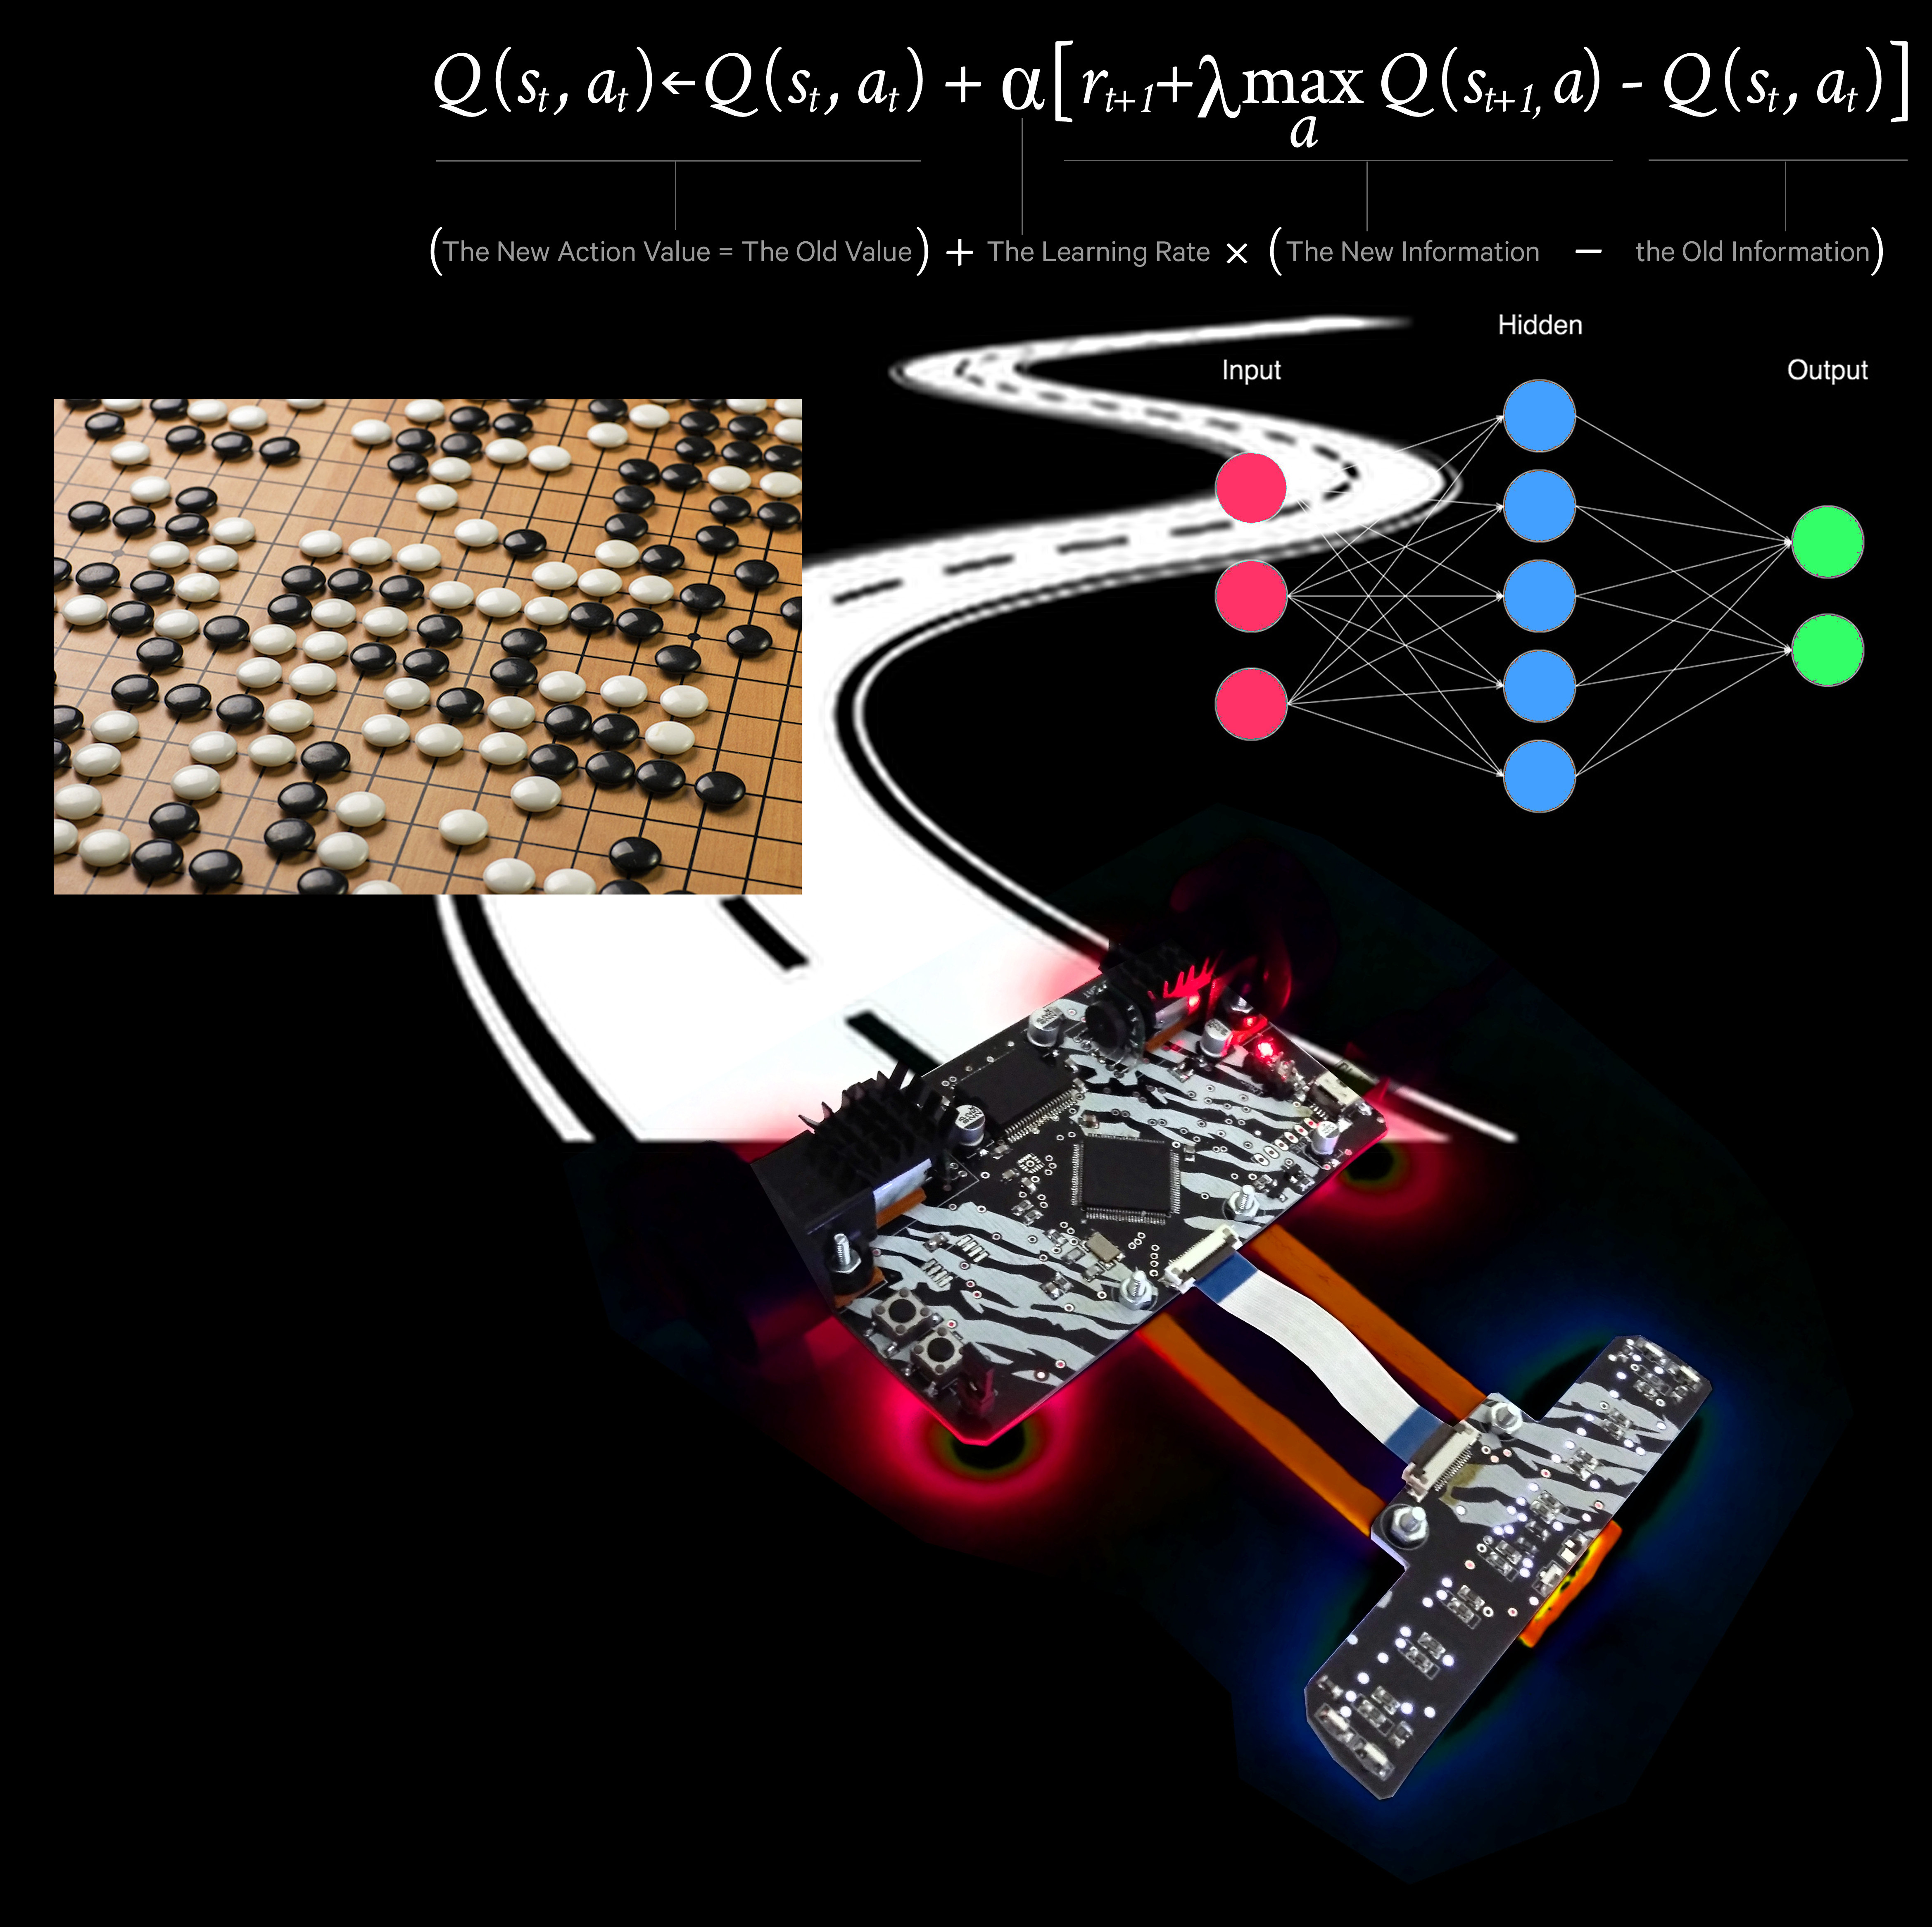
\includegraphics[width=5.05in]{../../pictures/rl_square.jpg}}

        \hfil}\vfil}
    }
    \begin{frame}

    %\titlepage


    \centering
     \colorbox{black}
     {
        \begin{minipage}{7cm}
           {\LARGE \color{white} \bf Image detection} \\
           {\LARGE \color{white} Michal CHOVANEC, PhD} \\
       \end{minipage}
     }


    \end{frame}
}

\begin{frame}{\bf Classification, Detection, Segmentation}

\begin{figure}
  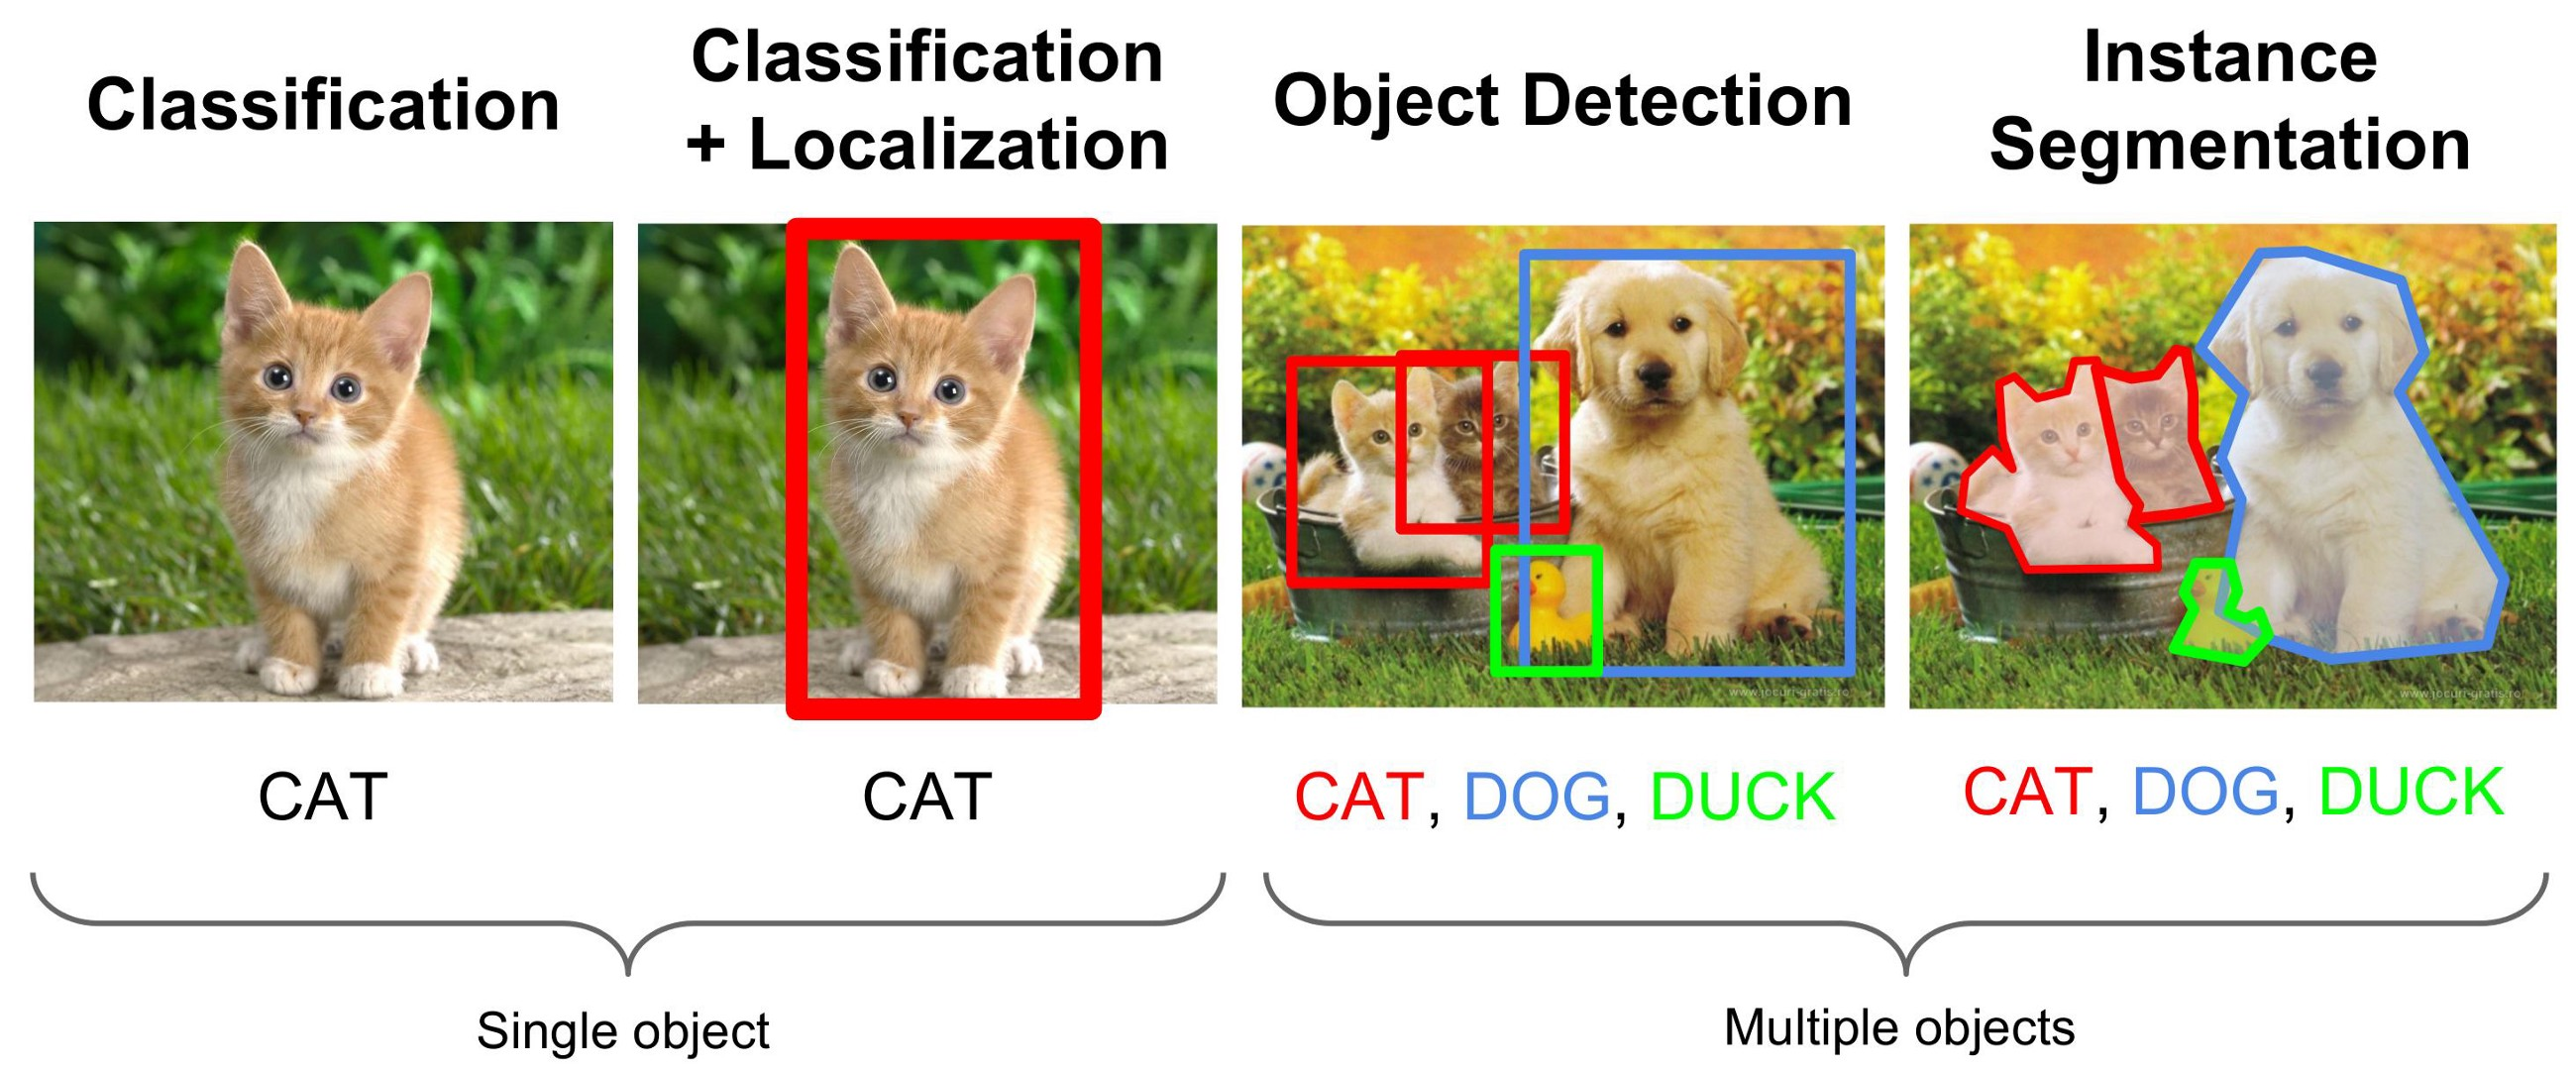
\includegraphics[scale=0.1]{../../pictures/cds.jpg}
\end{figure}

\end{frame}

\begin{frame}{\bf Historical methods}

    \begin{itemize}
        \item noise filtering
        \item edge detection
        \item thresholding
        \item histogram of oriented gradients, HOG, SVM
    \end{itemize}

\end{frame}

\begin{frame}{\bf Noise filtering}

\begin{columns}
\begin{column}{0.5\textwidth}

  \begin{figure}[!htb]
    \centering
    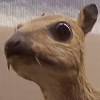
\includegraphics[scale=1.1]{../../pictures/image_processing/orig.png}
  \end{figure}

  \begin{figure}[!htb]
    \centering
    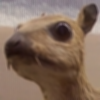
\includegraphics[scale=1.1]{../../pictures/image_processing/blur.png}
  \end{figure}

  \begin{figure}[!htb]
    \centering
    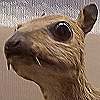
\includegraphics[scale=1.1]{../../pictures/image_processing/sharping.png}
  \end{figure}

\end{column}
\begin{column}{0.5\textwidth}  %%<--- here

  \scriptsize
  {
    \begin{align*}
    \begin{vmatrix}
        0 & 0 & 0 \\
        0 & 1 & 0 \\
        0 & 0 & 0 \\
    \end{vmatrix}\\
    \end{align*}
  }
  \scriptsize
  {
    \begin{align*}
    \begin{vmatrix}
        1 & 1 & 1 \\
        1 & 1 & 1 \\
        1 & 1 & 1 \\
    \end{vmatrix}\\
    \end{align*}
  }
  \scriptsize
  {
    \begin{align*}
    \begin{vmatrix}
        0 & -1 & 0 \\
        -1 & 5 & -1 \\
        0 & -1 & 0 \\
    \end{vmatrix}\\
    \end{align*}
  }
\end{column}
\end{columns}


{\tiny source \url{https://en.wikipedia.org/wiki/Kernel_(image_processing)}}

\end{frame}





\begin{frame}{\bf Edge detection}

\begin{columns}
\begin{column}{0.5\textwidth}

  \begin{figure}[!htb]
    \centering
    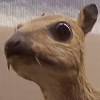
\includegraphics[scale=1.1]{../../pictures/image_processing/orig.png}
  \end{figure}

  \begin{figure}[!htb]
    \centering
    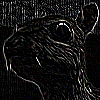
\includegraphics[scale=1.1]{../../pictures/image_processing/edges.png}
  \end{figure}

  \begin{figure}[!htb]
    \centering
    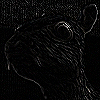
\includegraphics[scale=1.1]{../../pictures/image_processing/edges2.png}
  \end{figure}

\end{column}
\begin{column}{0.5\textwidth}  %%<--- here

  \scriptsize
  {
    \begin{align*}
    \begin{vmatrix}
        0 & 0 & 0 \\
        0 & 1 & 0 \\
        0 & 0 & 0 \\
    \end{vmatrix}\\
    \end{align*}
  }
  \scriptsize
  {
    \begin{align*}
    \begin{vmatrix}
        -1 & -1 & -1 \\
        -1 & 8 & -1 \\
        -1 & -1 & -1 \\
    \end{vmatrix}\\
    \end{align*}
  }
  \scriptsize
  {
    \begin{align*}
    \begin{vmatrix}
        0 & 1 & 0 \\
        1 & -4 & 1 \\
        0 & 1 & 0 \\
    \end{vmatrix}\\
    \end{align*}
  }
\end{column}
\end{columns}



{\tiny source \url{https://en.wikipedia.org/wiki/Kernel_(image_processing)}}

\end{frame}


\begin{frame}{\bf Thresholding}


\begin{figure}[!htb]
  \centering
  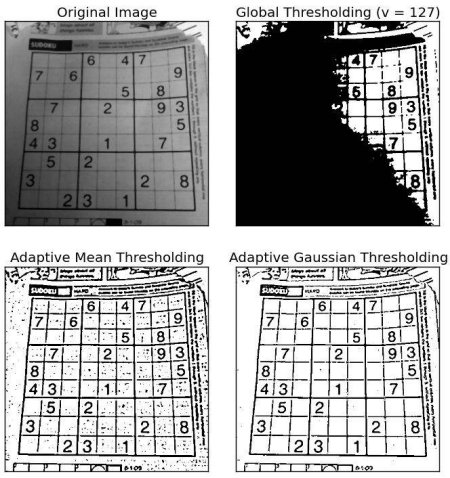
\includegraphics[scale=0.3]{../../pictures/image_processing/ada_threshold.jpg}
\end{figure}

{\tiny source \url{https://docs.opencv.org/3.4.3/d7/d4d/tutorial_py_thresholding.html}}

\end{frame}


\begin{frame}{\bf Histogram of oriented gradients}

\begin{figure}[!htb]
  \centering
  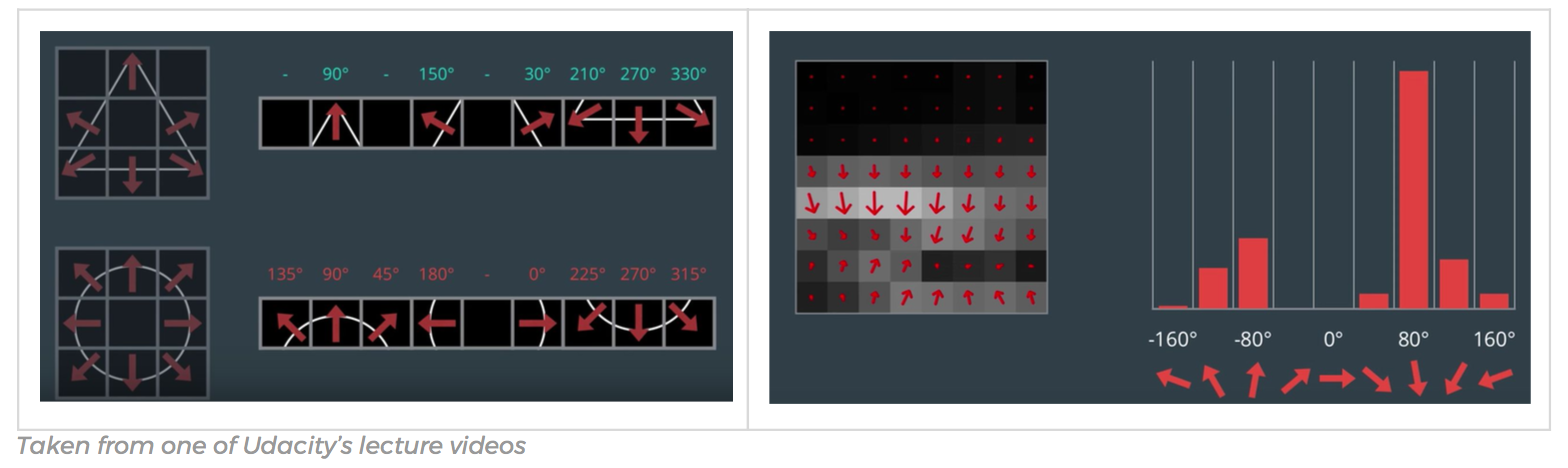
\includegraphics[scale=0.2]{../../pictures/image_processing/hog.png}
\end{figure}

\begin{figure}[!htb]
  \centering
  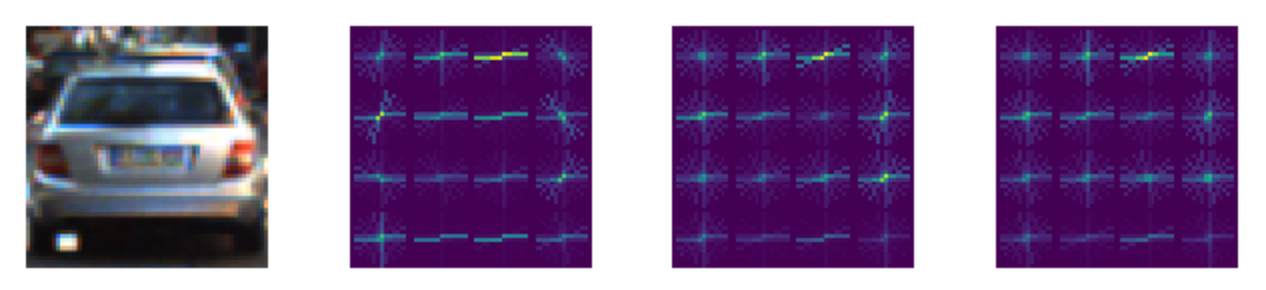
\includegraphics[scale=0.1]{../../pictures/image_processing/hog_car.png}
\end{figure}

\begin{figure}[!htb]
  \centering
  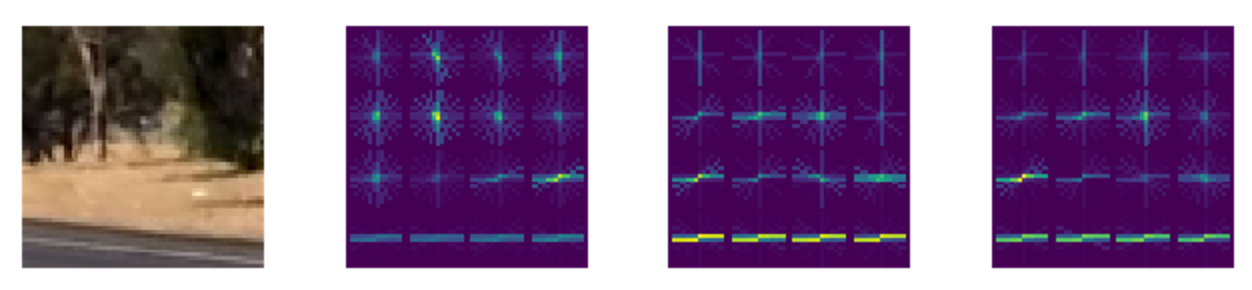
\includegraphics[scale=0.1]{../../pictures/image_processing/hog_no_car.png}
\end{figure}

{\tiny source \url{https://medium.com/@mithi/vehicles-tracking-with-hog-and-linear-svm-c9f27eaf521a}}

\end{frame}


\begin{frame}{\bf Deep neural networks}

\begin{enumerate}
    \item good dataset
        \begin{itemize}
            \item at least 10x images than network parameters
            \item random noised, shifted, rotated, luminance, resized
            \item {\bf \color{red} errors in dataset !}
        \end{itemize}

        \begin{figure}[!htb]
          \centering
          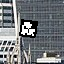
\includegraphics[scale=0.7]{../../pictures/image_processing/dataset_example/0.png}
          
\includegraphics[scale=0.7]{../../pictures/image_processing/dataset_example/1.png}
          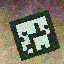
\includegraphics[scale=0.7]{../../pictures/image_processing/dataset_example/2.png}
          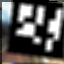
\includegraphics[scale=0.7]{../../pictures/image_processing/dataset_example/3.png}
        \end{figure}
    \item good CNN architecture
        \begin{itemize}
            \item convolution + pooling layers, full connected
            \item VGG net, YOLO
        \end{itemize}
\end{enumerate}

\end{frame}




\begin{frame}{\bf CNN architecture}

\begin{columns}
\begin{column}{0.5\textwidth}
    {\bf path net 0}
    \begin{itemize}
        \item C8-P2-C8-P2-C8-P2-FC2
        \item accuracy 95.856\%
        \item 1.840132 MFlops
        \item 65FPS, 640x480, GTX940
    \end{itemize}

    \begin{figure}[!htb]
      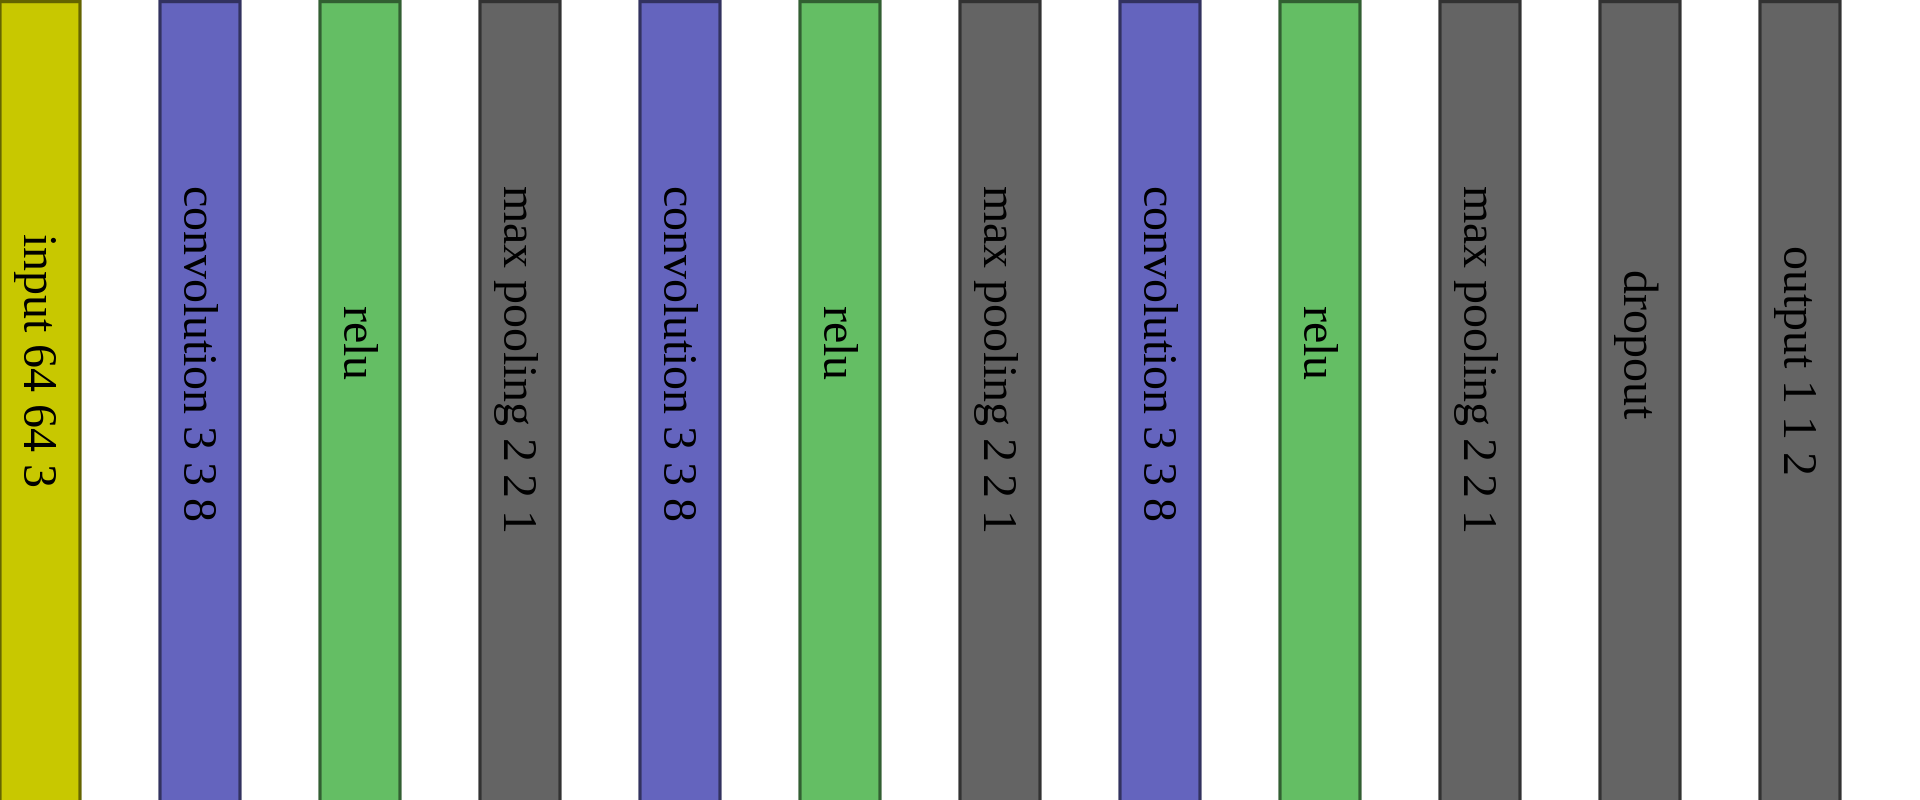
\includegraphics[scale=0.09]{../../pictures/image_processing/path_net_0.png}
    \end{figure}

\end{column}
\begin{column}{0.5\textwidth}  %%<--- here

    {\bf path net 3}
    \begin{itemize}
        \item C16-P2-C32-P2-C32-P2-FC2
        \item accuracy 97.01\%
        \item 9.392132 MFlops
        \item 18FPS, 640x480, GTX940
    \end{itemize}

    \begin{figure}[!htb]
      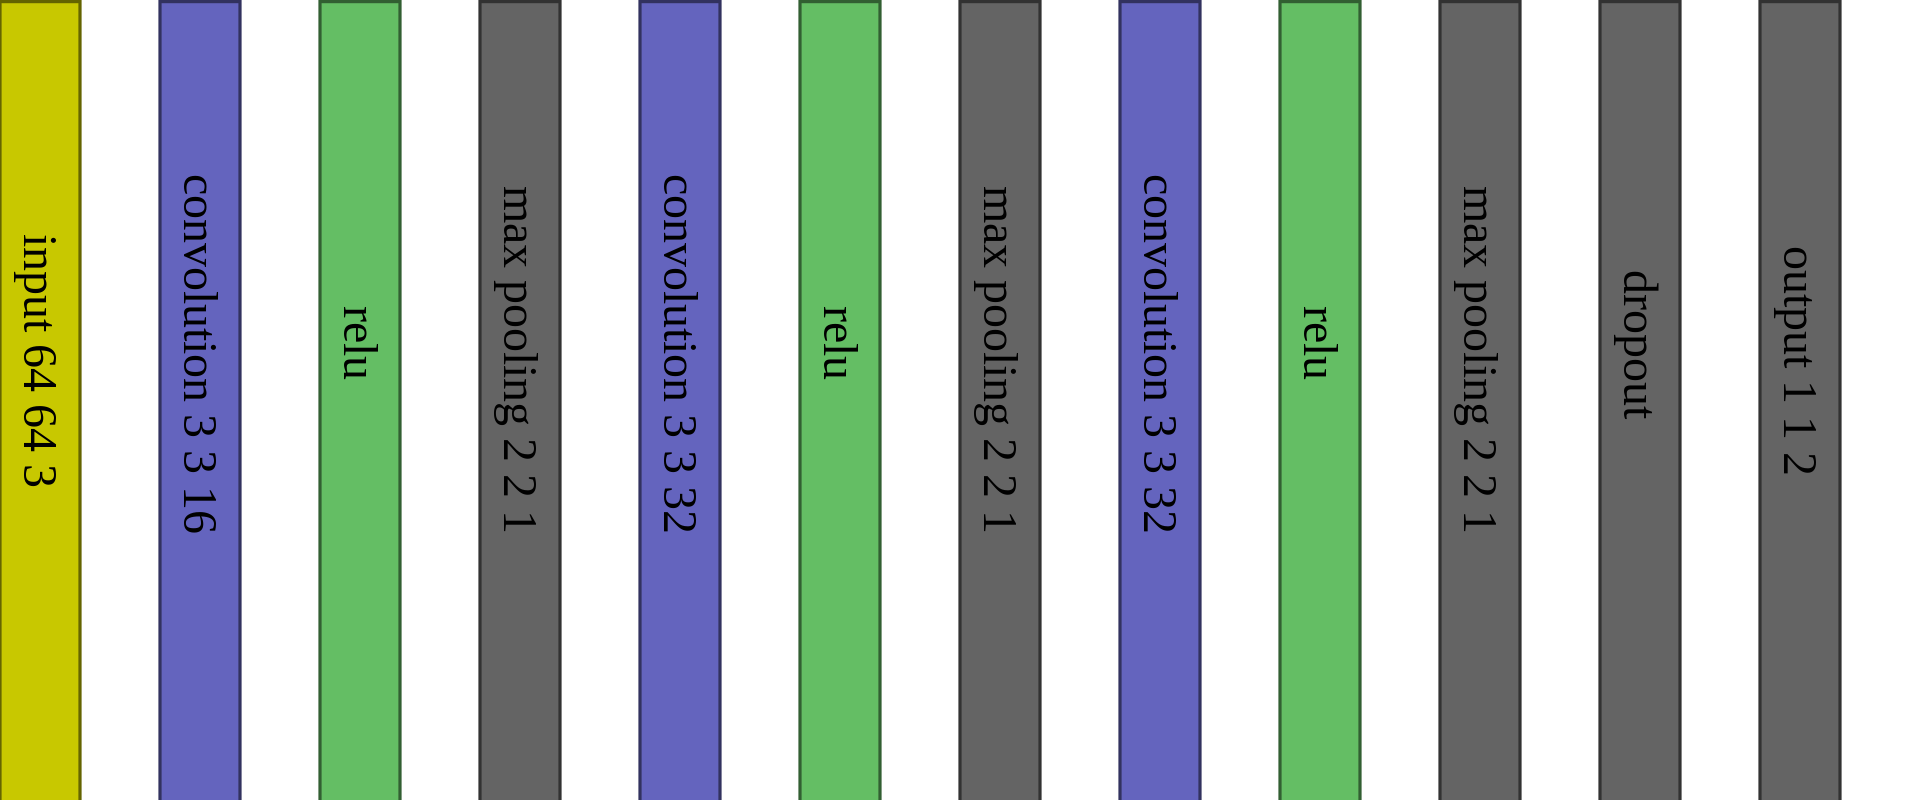
\includegraphics[scale=0.09]{../../pictures/image_processing/path_net_3.png}
    \end{figure}

\end{column}
\end{columns}

\end{frame}


\begin{frame}{\bf Deep neural network, detector mode}

\begin{figure}[!htb]
  \centering
  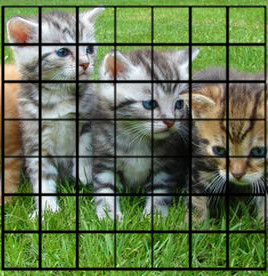
\includegraphics[scale=0.4]{../../pictures/image_processing/squared.jpg}
  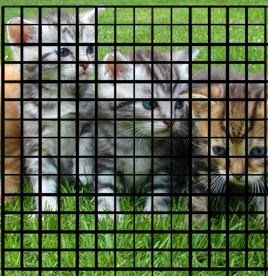
\includegraphics[scale=0.4]{../../pictures/image_processing/squared_overlap.jpg}
\end{figure}

\end{frame}


\begin{frame}{\bf Testing}

\begin{figure}[!htb]
  \centering
  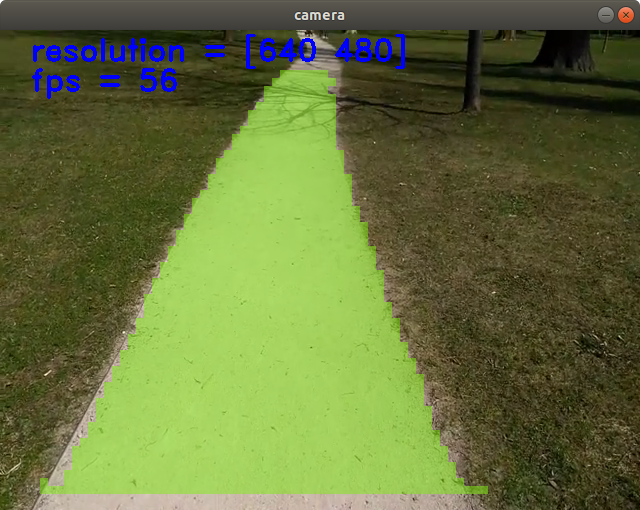
\includegraphics[scale=0.2]{../../pictures/image_processing/detector_test_0.png}
\end{figure}

\begin{figure}[!htb]
  \centering
  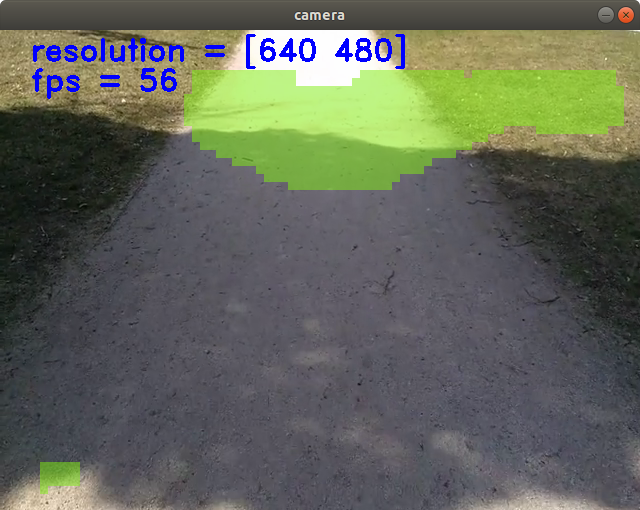
\includegraphics[scale=0.2]{../../pictures/image_processing/detector_test_1.png}
\end{figure}


\end{frame}




\begin{frame}{\bf Q\&A}

\begin{figure}
  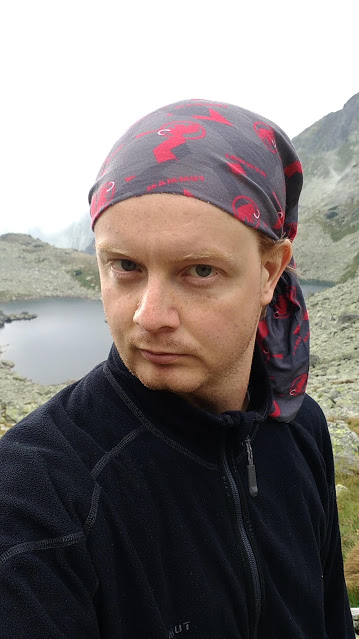
\includegraphics[scale=0.25]{../../pictures/me.jpg}
\end{figure}

\centering {
michal chovanec (michal.nand@gmail.com)
\url{www.youtube.com/channel/UCzVvP2ou8v3afNiVrPAHQGg}
}

\centering {
github
\url{https://github.com/michalnand}
}

\end{frame}


\end{document}
